% =============================================================================
% 構造塔の順序論的例示 — Lean 4 / Mathlib による形式化
% LuaLaTeX document
% =============================================================================
\documentclass[a4paper,11pt]{ltjsarticle}

% --- Core packages ---
\usepackage{luatexja-fontspec}
\usepackage{amsmath,amssymb,amsthm}
\usepackage{mathtools}
\usepackage{tikz-cd}
\usepackage{tikz}
\usetikzlibrary{arrows.meta,positioning,calc,decorations.pathmorphing,fit,shapes.geometric}
\usepackage{enumitem}
\usepackage{hyperref}
\usepackage{tcolorbox}
\tcbuselibrary{skins,breakable}
\usepackage{listings}
\usepackage{xcolor}
\usepackage{geometry}
\usepackage{fancyhdr}
\usepackage{float}
\usepackage{booktabs}

% --- Page geometry ---
\geometry{margin=2.5cm, top=3cm, bottom=3cm}

% --- Fonts ---
\setmainjfont{Harano Aji Mincho}
\setsansjfont{Harano Aji Gothic}

% --- Colors ---
\definecolor{leanblue}{HTML}{2563EB}
\definecolor{leanbg}{HTML}{F8FAFC}
\definecolor{leancomment}{HTML}{6B7280}
\definecolor{leankeyword}{HTML}{7C3AED}
\definecolor{leanstring}{HTML}{059669}
\definecolor{accentcolor}{HTML}{1E40AF}
\definecolor{theoremcolor}{HTML}{EFF6FF}
\definecolor{definitioncolor}{HTML}{F0FDF4}
\definecolor{remarkcolor}{HTML}{FFF7ED}
\definecolor{examplecolor}{HTML}{F0FDF4}

% --- Hyperref ---
\hypersetup{
  colorlinks=true,
  linkcolor=accentcolor,
  urlcolor=leanblue,
  citecolor=accentcolor,
  pdftitle={構造塔の順序論的例示},
  pdfauthor={su},
}

% --- Theorem environments ---
\theoremstyle{definition}
\newtheorem{definition}{定義}[section]
\newtheorem{example}[definition]{例}

\theoremstyle{plain}
\newtheorem{theorem}[definition]{定理}
\newtheorem{lemma}[definition]{補題}
\newtheorem{proposition}[definition]{命題}
\newtheorem{corollary}[definition]{系}

\theoremstyle{remark}
\newtheorem{remark}[definition]{注意}

% --- Lean code environment ---
\lstdefinelanguage{lean4}{
  morekeywords={def,theorem,lemma,example,instance,class,structure,
    where,let,in,do,if,then,else,match,with,fun,return,
    import,open,namespace,section,end,variable,
    inductive,abbrev,noncomputable,private,protected,
    sorry,admit,have,show,suffices,calc,by,exact,
    apply,intro,intros,constructor,cases,induction,
    simp,rw,rfl,ext,ring,linarith,omega,norm_num,
    decide,trivial,assumption,contradiction,rcases,
    Type,Prop,Sort,Set,true,false,attribute,
    monotone_level,union,level},
  sensitive=true,
  morecomment=[l]{--},
  morecomment=[n]{/-}{-/},
  morestring=[b]",
  literate=
    {α}{{\(\alpha\)}}1
    {β}{{\(\beta\)}}1
    {γ}{{\(\gamma\)}}1
    {ι}{{\(\iota\)}}1
    {κ}{{\(\kappa\)}}1
    {μ}{{\(\mu\)}}1
    {→}{{\(\to\)}}1
    {←}{{\(\leftarrow\)}}1
    {↔}{{\(\leftrightarrow\)}}1
    {≤}{{\(\leq\)}}1
    {≥}{{\(\geq\)}}1
    {≠}{{\(\neq\)}}1
    {∀}{{\(\forall\)}}1
    {∃}{{\(\exists\)}}1
    {∧}{{\(\wedge\)}}1
    {∨}{{\(\vee\)}}1
    {¬}{{\(\neg\)}}1
    {⊢}{{\(\vdash\)}}1
    {∈}{{\(\in\)}}1
    {∉}{{\(\notin\)}}1
    {⊆}{{\(\subseteq\)}}1
    {⊂}{{\(\subset\)}}1
    {∪}{{\(\cup\)}}1
    {∩}{{\(\cap\)}}1
    {∅}{{\(\emptyset\)}}1
    {⊤}{{\(\top\)}}1
    {⊥}{{\(\bot\)}}1
    {∘}{{\(\circ\)}}1
    {ℕ}{{\(\mathbb{N}\)}}1
    {ℤ}{{\(\mathbb{Z}\)}}1
    {ℝ}{{\(\mathbb{R}\)}}1
    {:=}{{:=}}2,
}

\lstnewenvironment{leancode}[1][]{%
  \lstset{
    language=lean4,
    basicstyle=\ttfamily\small,
    keywordstyle=\color{leankeyword}\bfseries,
    commentstyle=\color{leancomment}\itshape,
    stringstyle=\color{leanstring},
    backgroundcolor=\color{leanbg},
    frame=single,
    rulecolor=\color{leanblue!30},
    framesep=8pt,
    xleftmargin=12pt,
    xrightmargin=12pt,
    breaklines=true,
    breakatwhitespace=true,
    showstringspaces=false,
    tabsize=2,
    captionpos=b,
    numbers=left,
    numberstyle=\tiny\color{leancomment},
    numbersep=8pt,
    aboveskip=1em,
    belowskip=1em,
    escapeinside={(*}{*)},
    #1
  }%
}{}

% --- Tcolorbox styles ---
\newtcolorbox{proofstrategy}{
  colback=remarkcolor,
  colframe=orange!60!black,
  title={\textbf{証明戦略}},
  fonttitle=\sffamily,
  boxrule=0.5pt,
  arc=3pt,
}

\newtcolorbox{mathinsight}{
  colback=theoremcolor,
  colframe=accentcolor,
  title={\textbf{数学的洞察}},
  fonttitle=\sffamily,
  boxrule=0.5pt,
  arc=3pt,
}

\newtcolorbox{leaninsight}{
  colback=definitioncolor,
  colframe=leanblue!60!black,
  title={\textbf{Lean 実装のポイント}},
  fonttitle=\sffamily,
  boxrule=0.5pt,
  arc=3pt,
}

% --- Header/Footer ---
\pagestyle{fancy}
\fancyhf{}
\renewcommand{\headrulewidth}{0.4pt}
\fancyhead[L]{\small\sffamily\nouppercase{\leftmark}}
\fancyhead[R]{\small\sffamily 構造塔の形式化}
\fancyfoot[C]{\thepage}

% --- Custom macros ---
\newcommand{\ST}[2]{\mathsf{ST}(#1,\,#2)}
\newcommand{\Iic}{\mathrm{Iic}}
\newcommand{\Ici}{\mathrm{Ici}}
\newcommand{\Icc}{\mathrm{Icc}}
\newcommand{\lev}{\mathrm{level}}
\newcommand{\OD}{{}^{\mathrm{od}}}
\newcommand{\tlevel}[2]{T_{#1}.{\lev}(#2)}

% =============================================================================
\begin{document}

% --- Title ---
\title{%
  {\LARGE\sffamily\bfseries 構造塔の順序論的例示}\\[0.5em]
  {\large\sffamily Lean 4 / Mathlib による形式化とその数学的解説}%
}
\author{su}
\date{\today}
\maketitle

% --- AI Disclosure ---
\begin{center}
\small
\textit{AI assistance disclosure:}\\
Lean ソースコードは Claude (Anthropic) で骨格を生成し、
Claude Code (Anthropic) で修正した。\\
\TeX\ 文書は Claude Code (Anthropic) で生成した。\\
著者による加筆・修正は行っていない。\\
内容の正確性は保証されず、誤りがあれば著者の責任である。
\end{center}

\vspace{1em}

% --- Abstract ---
\begin{abstract}
ニコラ・ブルバキの「一般から特殊へ」という原則に倣い,
前順序集合で添字付けられた集合の単調な族(\textbf{構造塔}; structure tower)を
Lean~4 / Mathlib4 で形式化する.
定数塔・主下方集合塔($\Iic$ 塔)・主上方集合塔($\Ici$ 塔)・単調列塔・
自然数フィルトレーション・添字変換(函手性)・反単調族の双対化・
反復作用素塔・有界区間塔,ならびにレベルごとの積・交叉・合併,
の 12 種の例を系統的に与える.
さらに「単調列塔は $\Iic$ 塔の添字変換である」「有界区間塔は定数塔と $\Iic$ 塔の交叉である」
という例間の関係を定理として証明する.
形式化上の重要な技術的考察(strict implicit 引数の束縛,
\texttt{Function.iterate} の定義方向,\texttt{@[ext]} の登録)についても記述する.
\end{abstract}

\tableofcontents
\newpage

% =============================================================================
\section{はじめに}
% =============================================================================

ニコラ・ブルバキ(Nicolas Bourbaki)の数学原論(\textit{Éléments de mathématiques})は,
数学のあらゆる分野を「構造の種」(\textit{espèce de structures})という統一的な概念の
特殊化として再構成した.この哲学の核心は,まず最も抽象的な構造を定義し,
次第に条件を加えることで具体的な数学的対象を導くという方法論にある.

本文書では,この精神に従い,\textbf{前順序集合で添字付けられた集合の単調な族}
を「構造塔」(structure tower)と呼び,Lean~4 / Mathlib4 で形式化する.
構造塔は実質的には「前順序 $(\iota, \leq)$ から冪集合半順序 $(\mathcal{P}(\alpha), \subseteq)$
への単調写像」に過ぎないが,この抽象化が順序論・位相論・代数など広範な数学的対象を
統一的に記述することを,多彩な例示によって示す.

形式化の環境は以下の通りである:
\begin{itemize}
  \item \textbf{言語}:Lean~4(バージョン 4.28.0)
  \item \textbf{ライブラリ}:Mathlib4(\texttt{import Mathlib.Data.Set.Lattice},
        \texttt{Mathlib.Order.GaloisConnection.Basic},\texttt{Mathlib.Order.Closure})
  \item \textbf{名前空間}:\texttt{BourbakiGuide}
\end{itemize}

% =============================================================================
\section{構造塔の定義}
\label{sec:definition}
% =============================================================================

\subsection{定義と外延性}

\begin{definition}[構造塔]
\label{def:structure-tower}
前順序集合 $\iota$(添字集合)と集合 $\alpha$(台集合)に対して,
\textbf{構造塔} $T \in \ST{\iota}{\alpha}$ とは,
写像 $T.\lev : \iota \to \mathcal{P}(\alpha)$ であって,
\[
  i \leq j \implies T.\lev(i) \subseteq T.\lev(j)
\]
を満たすものである.
\end{definition}

図~\ref{fig:tower-concept} に構造塔の概念を示す.

\begin{figure}[H]
\centering
\begin{tikzcd}[column sep=4em, row sep=2.5em]
  {(\iota,\,\leq)} \arrow[r, "\lev", "\text{単調写像}"']
    & {(\mathcal{P}(\alpha),\,\subseteq)} \\
  i \arrow[r, mapsto] \arrow[d, "\leq"', sloped, phantom]
    & T.\lev(i) \arrow[d, "\subseteq", sloped, phantom] \\
  j \arrow[r, mapsto]
    & T.\lev(j)
\end{tikzcd}
\caption{構造塔は前順序から冪集合半順序への単調写像.
  $i \leq j$ ならば $T.\lev(i) \subseteq T.\lev(j)$.}
\label{fig:tower-concept}
\end{figure}

\begin{proposition}[外延性]
\label{prop:ext}
$T_1.\lev = T_2.\lev$ ならば $T_1 = T_2$.
\end{proposition}

\begin{remark}
Lean 4 の \texttt{@[ext]} 属性により,$\lev$ フィールドの等しさから
塔全体の等しさが自動的に導かれる.\texttt{monotone\_level} は命題型(Prop)なので,
証明無関係性(proof irrelevance)により \texttt{@[ext]} の生成に寄与しない.
\end{remark}

Lean でのコア定義:

\begin{leancode}[caption={StructureTower の定義と合併}]
@[ext]
structure StructureTower ((*$\iota$*) (*$\alpha$*) : Type*) [Preorder (*$\iota$*)] : Type _ where
  level   : (*$\iota$*) (*$\to$*) Set (*$\alpha$*)
  monotone_level : (*$\forall$*) (*$\langle\!\langle$*)i j : (*$\iota$*)(*$\rangle\!\rangle$*), i (*$\leq$*) j (*$\to$*) level i (*$\subseteq$*) level j

-- 塔が覆う全体集合
def union (T : StructureTower (*$\iota$*) (*$\alpha$*)) : Set (*$\alpha$*) :=
  (*$\bigcup$*) i, T.level i
\end{leancode}

\begin{leaninsight}
\textbf{strict implicit 引数}(\texttt{(*$\langle\!\langle$*)i j : (*$\iota$*)(*$\rangle\!\rangle$*)} )について:
Lean 4 の \texttt{(*$\langle\!\langle\cdot\rangle\!\rangle$*)}(二重山括弧)は「厳密暗黙引数」(strict implicit)を表す.
これは \texttt{\{\ \}} と異なり,lambda 式の中でも自動的にスキップされず,
明示的に束縛する必要がある.
例えば \texttt{monotone\_level} の証明は \texttt{fun \_i \_j hij \_x hx => ...} と
全引数を明示的に書く必要がある(単に \texttt{fun hij =>} と書くと \texttt{hij} が
添字 $i$ を束縛してしまいエラーになる).
\end{leaninsight}

\subsection{合併}

\begin{definition}[塔の合併]
塔 $T \in \ST{\iota}{\alpha}$ の\textbf{合併}(union)を
$T.\mathrm{union} := \bigcup_{i \in \iota} T.\lev(i)$
と定める.
\end{definition}

合併は「塔が記述する空間全体」を表す.後の定理で見るように,
$\Iic$ 塔の合併は台集合全体 $\alpha$ と一致する.

% =============================================================================
\section{基本例}
\label{sec:basic}
% =============================================================================

\subsection{定数塔}
\label{sec:const}

\begin{example}[定数塔 \texttt{const}]
\label{ex:const}
集合 $S \subseteq \alpha$ に対し,すべてのレベルで同じ集合 $S$ を返す塔:
\[
  \mathrm{const}(\iota, S).\lev(i) = S \quad (\forall i \in \iota)
\]
これは層別化の情報をまったく持たない退化的な極端例である.
\end{example}

\begin{leancode}[caption={定数塔 const}]
def const ((*$\iota$*) : Type*) [Preorder (*$\iota$*)] (S : Set (*$\alpha$*)) :
    StructureTower (*$\iota$*) (*$\alpha$*) where
  level _     := S
  monotone_level := fun _i _j _hij => Subset.refl _
-- 単調性:S ⊆ S(自明)

@[simp] theorem const_level (S : Set (*$\alpha$*)) (i : (*$\iota$*)) :
    (const (*$\iota$*) S).level i = S := rfl

theorem const_union (S : Set (*$\alpha$*)) [Nonempty (*$\iota$*)] :
    (const (*$\iota$*) S).union = S := by simp [union, Set.iUnion_const]
\end{leancode}

\subsection{主下方集合塔と主上方集合塔}
\label{sec:iic-ici}

主下方集合塔は,順序構造そのものを塔として見る最も基本的な例である.

\begin{example}[主下方集合塔 \texttt{iic}]
\label{ex:iic}
前順序集合 $\alpha$ に対し,
\[
  \Iic_\alpha.\lev(x) = \{y \in \alpha \mid y \leq x\} = (-\infty, x]
\]
これは「$\alpha$ を添字集合かつ台集合とする自己参照的な塔」であり,
塔 $\mathit{と}$ 順序関係が一致する.
\end{example}

\begin{theorem}[\texttt{iic} の合併]
\label{thm:iic-union}
任意の前順序集合 $\alpha$ に対して $(\Iic_\alpha).\mathrm{union} = \alpha$(全体集合).
\end{theorem}
\begin{proof}
任意の $x \in \alpha$ に対し,$x \in \Iic_\alpha.\lev(x)$(反射性 $x \leq x$).
ゆえに $x \in \bigcup_{i} \Iic_\alpha.\lev(i)$.
\end{proof}

\begin{example}[主上方集合塔 \texttt{ici}]
\label{ex:ici}
\[
  \Ici_\alpha.\lev(x) = \{y \in \alpha \mid x \leq y\} = [x, +\infty)
\]
ただし添字集合は $\alpha$ ではなく $\alpha^{\mathrm{od}}$(双対前順序)として,
塔の単調性を保証する:$\alpha^{\mathrm{od}}$ での $i \leq j$ は $\alpha$ での $j \leq i$ を意味する.
\end{example}

\begin{figure}[H]
\centering
\begin{tikzcd}[column sep=4em, row sep=3em]
  {(\alpha, \leq)} \arrow[r, "\Iic", bend left=15]
    \arrow[d, "\mathrm{dual}"']
    & \ST{\alpha}{\alpha} \arrow[d, dashed, "\text{同じ塔}" description] \\
  {(\alpha^{\mathrm{od}}, \leq^{\mathrm{od}})} \arrow[r, "\Ici", bend right=15]
    & \ST{\alpha^{\mathrm{od}}}{\alpha}
\end{tikzcd}
\caption{$\Iic$ 塔と $\Ici$ 塔の対称性.
  $\alpha^{\mathrm{od}}$ での $i \leq j$ は $\alpha$ での $j \leq i$ を意味し,
  $\Ici$ の単調性を保証する($j \leq i$ ならば $[i,\infty) \subseteq [j,\infty)$).}
\label{fig:iic-ici-duality}
\end{figure}

\begin{leancode}[caption={主下方集合塔 iic と主上方集合塔 ici}]
-- 主下方集合塔:level x = {y | y (*$\leq$*) x}
def iic ((*$\alpha$*) : Type*) [Preorder (*$\alpha$*)] : StructureTower (*$\alpha$*) (*$\alpha$*) where
  level x := Set.Iic x
  monotone_level := fun _i _j hij _x hx => le_trans hx hij
-- y (*$\leq$*) i (*$\leq$*) j より y (*$\leq$*) j:le_trans による推移律

-- 主上方集合塔(添字は (*$\alpha^{\mathrm{od}}$*)):level x = {y | ofDual(x) (*$\leq$*) y}
def ici ((*$\alpha$*) : Type*) [Preorder (*$\alpha$*)] : StructureTower (*$\alpha$*)(*${}^{\mathrm{od}}$*) (*$\alpha$*) where
  level x := Set.Ici (OrderDual.ofDual x)
  monotone_level := by
    intro i j hij y hy
    -- hij : i (*$\leq$*) j in (*$\alpha^{\mathrm{od}}$*) means ofDual j (*$\leq$*) ofDual i in (*$\alpha$*)
    exact le_trans (OrderDual.ofDual_le_ofDual.mpr hij) hy
\end{leancode}

\begin{mathinsight}
$\Iic$ 塔の単調性:$i \leq j$ ならば $\Iic(i) \subseteq \Iic(j)$.
これは $y \leq i \leq j$ の推移律そのものである.
一方 $\Ici$ 塔は「上方集合は $x$ が大きくなるほど小さくなる(下方単調)」ため,
添字集合を $\alpha^{\mathrm{od}}$(双対前順序)に取り替えることで上方単調にする.
$\alpha^{\mathrm{od}}$ での $i \leq j$ は $\alpha$ での $j \leq i$(すなわち
$\mathrm{ofDual}(j) \leq \mathrm{ofDual}(i)$)を意味する.
ゆえに $[{\mathrm{ofDual}(i)}, \infty) \supseteq [\mathrm{ofDual}(j), \infty)$,
つまり $\Ici.\lev(j) \subseteq \Ici.\lev(i)$... ではなく,
$\alpha^{\mathrm{od}}$ での $i \leq j$ から $\Ici.\lev(i) \subseteq \Ici.\lev(j)$ が従う.
\end{mathinsight}

% =============================================================================
\section{列による例}
\label{sec:seq}
% =============================================================================

\subsection{単調列塔}
\label{sec:monotone-seq}

\begin{example}[単調列塔 \texttt{ofMonotoneSeq}]
単調な列 $c : \mathbb{N} \to \alpha$(すなわち $m \leq n \Rightarrow c(m) \leq c(n)$)から,
\[
  \mathrm{ofMonotoneSeq}(c, h_c).\lev(n) = \{y \mid y \leq c(n)\} = \Iic(c(n))
\]
を構成する.これは「$n$ 段目の截断 $(-\infty, c(n)]$」を積み上げたフィルトレーションである.
\end{example}

\begin{example}[自然数フィルトレーション \texttt{natFiltration}]
\label{ex:nat-filtration}
$c = \mathrm{id} : \mathbb{N} \to \mathbb{N}$ を単調列として得られる標準的なフィルトレーション:
\[
  \mathrm{natFiltration}.\lev(n) = \{m \in \mathbb{N} \mid m \leq n\} = [0, n]
\]
$\mathrm{natFiltration}.\mathrm{union} = \mathbb{N}$(全体)となる($\forall n,\, n \in [0,n]$).
\end{example}

\begin{leancode}[caption={単調列塔と自然数フィルトレーション}]
def ofMonotoneSeq {(*$\alpha$*) : Type*} [Preorder (*$\alpha$*)]
    (c : (*$\mathbb{N}$*) (*$\to$*) (*$\alpha$*)) (hc : Monotone c) :
    StructureTower (*$\mathbb{N}$*) (*$\alpha$*) where
  level n     := Set.Iic (c n)   -- 截断 ((*$-\infty$*), c(n)]
  monotone_level := fun _i _j hij _x hx => le_trans hx (hc hij)
-- y (*$\leq$*) c(i) (*$\leq$*) c(j)(hc hij : c(i) (*$\leq$*) c(j))

-- 特例:c = id
def natFiltration : StructureTower (*$\mathbb{N}$*) (*$\mathbb{N}$*) :=
  ofMonotoneSeq id monotone_id

-- 合併 = (*$\mathbb{N}$*) 全体
theorem natFiltration_union_eq_univ :
    natFiltration.union = Set.univ := by
  apply Set.eq_univ_of_forall
  intro x
  simp only [union, natFiltration, ofMonotoneSeq, Set.mem_iUnion, Set.mem_Iic, id]
  exact (*$\langle$*)x, le_refl x(*$\rangle$*)  -- 証人:i = x,証明:x (*$\leq$*) x
\end{leancode}

% =============================================================================
\section{添字変換(函手性)}
\label{sec:reindex}
% =============================================================================

\begin{definition}[添字変換 \texttt{reindex}]
前順序集合の単調写像 $f : \iota \to \kappa$ と塔 $T \in \ST{\kappa}{\alpha}$ から,
$\iota$ で添字付けられた塔を
\[
  (\mathrm{reindex}\,f\,T).\lev(i) := T.\lev(f(i))
\]
と定める.
\end{definition}

\begin{figure}[H]
\centering
\begin{tikzcd}[column sep=3.5em, row sep=2.5em]
  {(\iota, \leq_\iota)} \arrow[r, "f"] \arrow[dr, "\mathrm{reindex}\,f\,T"']
    & {(\kappa, \leq_\kappa)} \arrow[d, "T.\lev"] \\
    & {(\mathcal{P}(\alpha), \subseteq)}
\end{tikzcd}
\caption{添字変換の函手性:$\mathrm{reindex}\,f\,T$ は $T.\lev \circ f$ に等しい.
  $f$ が単調かつ $T$ が単調ならば合成も単調.}
\label{fig:reindex}
\end{figure}

これは「塔の圏における引き戻し(pullback)」であり,函手的な性質を持つ:

\begin{theorem}[添字変換の函手性]
\label{thm:reindex-functorial}
\begin{enumerate}[label=(\roman*)]
  \item $\mathrm{reindex}\,\mathrm{id}\,T = T$(恒等律)
  \item $\mathrm{reindex}\,f\,(\mathrm{reindex}\,g\,T) = \mathrm{reindex}\,(g \circ f)\,T$(合成律)
\end{enumerate}
\end{theorem}

\begin{leancode}[caption={添字変換と函手性}]
def reindex {(*$\kappa$*) : Type*} [Preorder (*$\kappa$*)]
    (f : (*$\iota$*) (*$\to$*) (*$\kappa$*)) (hf : Monotone f)
    (T : StructureTower (*$\kappa$*) (*$\alpha$*)) : StructureTower (*$\iota$*) (*$\alpha$*) where
  level i          := T.level (f i)    -- 合成 T.lev (*$\circ$*) f
  monotone_level := fun _i _j hij => T.monotone_level (hf hij)

-- 恒等律:reindex id = id
theorem reindex_id (T : StructureTower (*$\iota$*) (*$\alpha$*)) :
    reindex id monotone_id T = T := by ext i _; simp

-- 合成律(函手性)
theorem reindex_comp
    (f : (*$\iota$*) (*$\to$*) (*$\kappa$*)) (hf : Monotone f)
    (g : (*$\kappa$*) (*$\to$*) (*$\mu$*)) (hg : Monotone g)
    (T : StructureTower (*$\mu$*) (*$\alpha$*)) :
    reindex f hf (reindex g hg T) = reindex (g (*$\circ$*) f) (hg.comp hf) T := by
  ext i _; simp
\end{leancode}

\begin{mathinsight}
\texttt{reindex} は「塔の圏 $\ST{-}{\alpha}$」における前引き(pullback)函手の作用である.
これを用いると,例えば単調列塔と $\Iic$ 塔の関係を明確に述べることができる
(定理~\ref{thm:seq-is-reindex}).
\end{mathinsight}

% =============================================================================
\section{双対化と反復作用素塔}
\label{sec:dual-iterate}
% =============================================================================

\subsection{反単調族の双対化}
\label{sec:antitone}

\begin{example}[反単調族の双対化 \texttt{ofAntitone}]
\textbf{反単調}(antitone)な族 $d : \iota \to \mathcal{P}(\alpha)$($i \leq j \Rightarrow d(j) \subseteq d(i)$)は,
添字集合を $\iota^{\mathrm{od}}$ に替えることで単調な族(=塔)になる:
\[
  \mathrm{ofAntitone}(d, h_d).\lev^{\iota^{\mathrm{od}}}(i) := d(\mathrm{ofDual}(i))
\]
\end{example}

これは $\Ici$ 塔の一般化:$\Ici$ は $x \mapsto [x, \infty)$ という反単調族から構成される.

\begin{leancode}[caption={反単調族の双対化}]
def ofAntitone (d : (*$\iota$*) (*$\to$*) Set (*$\alpha$*)) (hd : Antitone d) :
    StructureTower (*$\iota$*)(*${}^{\mathrm{od}}$*) (*$\alpha$*) where
  level i := d (OrderDual.ofDual i)
  monotone_level := by
    intro i j hij
    -- i (*$\leq$*) j in (*$\iota^{\mathrm{od}}$*) (*$\Rightarrow$*) ofDual j (*$\leq$*) ofDual i in (*$\iota$*)
    exact hd (OrderDual.ofDual_le_ofDual.mpr hij)
\end{leancode}

\subsection{反復作用素塔}
\label{sec:iterate}

\begin{example}[反復作用素塔 \texttt{ofIterate}]
単調写像 $f : \mathcal{P}(\alpha) \to \mathcal{P}(\alpha)$ と $S \subseteq f(S)$(膨張的)を満たす集合 $S$ から,
\[
  \mathrm{ofIterate}(f, h_f, S, h_{\mathrm{exp}}).\lev(n) := f^n(S) \quad (n \in \mathbb{N})
\]
を構成する.これは「生成列」「反復閉包」「$\sigma$-代数の段階的構成」等をモデル化する.
\end{example}

\begin{figure}[H]
\centering
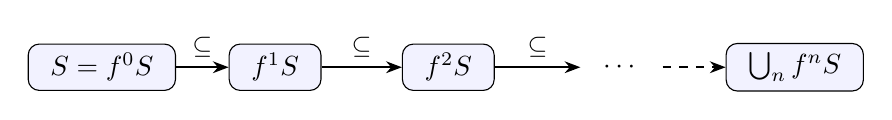
\begin{tikzpicture}[node distance=2.2cm,
  every node/.style={draw, rounded corners=4pt, fill=blue!5,
    minimum height=1.4em, inner xsep=8pt}]
  \node (S0) {$S = f^0 S$};
  \node (S1) [right of=S0] {$f^1 S$};
  \node (S2) [right of=S1] {$f^2 S$};
  \node (Sdot) [right of=S2, draw=none, fill=none] {$\cdots$};
  \node (Su) [right of=Sdot] {$\bigcup_n f^n S$};

  \draw[-{Stealth}, semithick] (S0) -- node[above, draw=none, fill=none]
    {\small $\subseteq$} (S1);
  \draw[-{Stealth}, semithick] (S1) -- node[above, draw=none, fill=none]
    {\small $\subseteq$} (S2);
  \draw[-{Stealth}, semithick] (S2) -- node[above, draw=none, fill=none]
    {\small $\subseteq$} (Sdot);
  \draw[-{Stealth}, semithick, dashed] (Sdot) -- (Su);
\end{tikzpicture}
\caption{反復作用素塔:$S \subseteq f(S) \subseteq f^2(S) \subseteq \cdots$.
  膨張的かつ単調な $f$ のもと,反復列は $\mathbb{N}$-塔をなす.}
\label{fig:iterate-chain}
\end{figure}

\begin{leancode}[caption={反復作用素塔とその補助補題}]
-- 補助:膨張的単調 f では f^[n](S) (*$\subseteq$*) f^[n+1](S)
private theorem iterate_subset_succ
    (f : Set (*$\alpha$*) (*$\to$*) Set (*$\alpha$*)) (hf : Monotone f)
    (S : Set (*$\alpha$*)) (hS : S (*$\subseteq$*) f S) :
    (*$\forall$*) n : (*$\mathbb{N}$*), f^[n] S (*$\subseteq$*) f^[n + 1] S := by
  intro n
  induction n with
  | zero => exact hS        -- f^0 S = S (*$\subseteq$*) f S = f^1 S
  | succ k ih =>
    -- 注:Lean 4 の iterate は f^[n+1] x = f^[n](f(x)) と定義される(左再帰)
    -- 定理的等号 f^[n+1] = f (*$\circ$*) f^[n] を使う
    simp only [Function.iterate_succ', Function.comp] at ih (*$\vdash$*)
    exact hf ih  -- f 単調性により f(f^[k] S) (*$\subseteq$*) f(f^[k+1] S)

def ofIterate (f : Set (*$\alpha$*) (*$\to$*) Set (*$\alpha$*)) (hf : Monotone f)
    (S : Set (*$\alpha$*)) (hexpand : S (*$\subseteq$*) f S) :
    StructureTower (*$\mathbb{N}$*) (*$\alpha$*) where
  level n := f^[n] S
  monotone_level := by
    intro i j hij
    induction hij with
    | refl => exact Subset.rfl     -- i = j のとき自明
    | step _ ih =>
      exact Subset.trans ih (iterate_subset_succ f hf S hexpand _)
\end{leancode}

\begin{proofstrategy}
\texttt{iterate\_subset\_succ} の帰納法:
\begin{itemize}
  \item 基底:$f^0 S = S \subseteq f(S) = f^1 S$(膨張条件 \texttt{hS})
  \item 帰納段:$f^k S \subseteq f^{k+1} S$ を仮定(IH)し,
        $f^{k+1} S \subseteq f^{k+2} S$ を示す.
        \texttt{Function.iterate\_succ'} により $f^{k+1} = f \circ f^k$ と書き直し,
        $f$ の単調性(\texttt{hf ih})を適用する.
\end{itemize}
IH (\texttt{ih}) と目標を同時に書き換えるため \texttt{at ih (*$\vdash$*)} が必要.
\end{proofstrategy}

\begin{leaninsight}
Lean 4 における \texttt{Function.iterate} の定義は:\\
\texttt{f\^{}[0] x = x},\quad \texttt{f\^{}[n+1] x = f\^{}[n](f(x))}(左再帰・右適用)\\
であり,$f^{n+1} x = f(f^n x)$(右再帰・左適用)とは\textbf{命題的に等しいが定義的に異なる}.
\texttt{show f(f\^{}[k] S) (*$\subseteq$*) f(f\^{}[k+1] S)} と書くと
``not definitionally equal'' エラーになる.
\texttt{simp only [Function.iterate\_succ', Function.comp]} で書き換えてから証明する必要がある.
\end{leaninsight}

% =============================================================================
\section{有界区間塔}
\label{sec:icc}
% =============================================================================

\begin{example}[有界区間塔 \texttt{icc}]
\label{ex:icc}
下界 $a \in \alpha$ に対し,
\[
  \Icc_a.\lev(x) = \{y \mid a \leq y \leq x\} = [a, x]
\]
これは $\Iic$ 塔を下から $a$ で切り取った「有界版」である.
\end{example}

\begin{theorem}[\texttt{icc} と \texttt{iic} の包含関係]
$\Icc_a.\lev(x) \subseteq \Iic_\alpha.\lev(x)$(下界付き区間は通常区間に含まれる).
\end{theorem}

\begin{leancode}[caption={有界区間塔}]
def icc {(*$\alpha$*) : Type*} [Preorder (*$\alpha$*)] (a : (*$\alpha$*)) :
    StructureTower (*$\alpha$*) (*$\alpha$*) where
  level x := Set.Icc a x           -- [a, x]
  monotone_level := fun _i _j hij _y hy =>
    (*$\langle$*)hy.1, le_trans hy.2 hij(*$\rangle$*)
  -- hy : a (*$\leq$*) y (*$\wedge$*) y (*$\leq$*) i,hij : i (*$\leq$*) j より y (*$\leq$*) j

theorem icc_level_subset_iic_level (a x : (*$\alpha$*)) :
    (icc a).level x (*$\subseteq$*) (iic (*$\alpha$*)).level x :=
  fun _ hy => hy.2    -- hy.2 : y (*$\leq$*) x
\end{leancode}

% =============================================================================
\section{レベルごとの構成}
\label{sec:levelwise}
% =============================================================================

塔の間の自然な演算として,積・交叉・合併(レベルごとの)を定義できる.

\begin{definition}[レベルごとの演算]
塔 $T_1 \in \ST{\iota}{\alpha}$,$T_2 \in \ST{\iota}{\beta}$ に対し:
\begin{align*}
  (\mathrm{prod}\,T_1\,T_2).\lev(i) &:= T_1.\lev(i) \times T_2.\lev(i) \subseteq \alpha \times \beta\\
  (\mathrm{inter}\,T_1\,T_2).\lev(i) &:= T_1.\lev(i) \cap T_2.\lev(i) \subseteq \alpha \quad (T_2 \in \ST{\iota}{\alpha})\\
  (\mathrm{sup}\,T_1\,T_2).\lev(i) &:= T_1.\lev(i) \cup T_2.\lev(i) \subseteq \alpha
\end{align*}
いずれも,$i \leq j$ での単調性はレベルごとに引き継がれる.
\end{definition}

\begin{figure}[H]
\centering
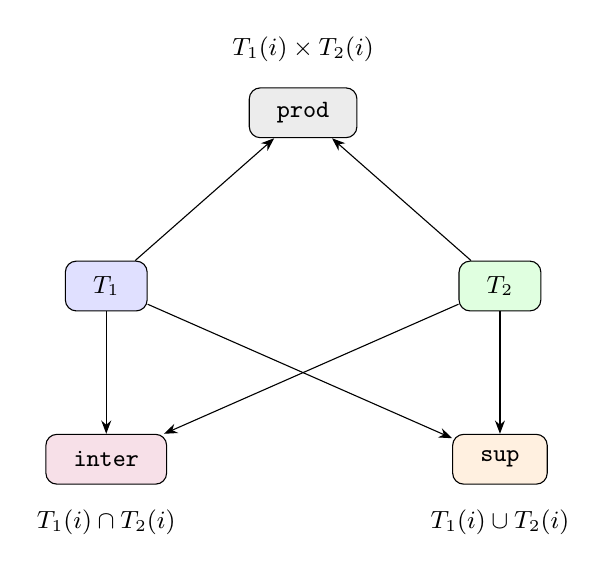
\begin{tikzpicture}[
  box/.style={draw, rounded corners=4pt, minimum height=1.8em,
              inner xsep=10pt, font=\small}]
  % 入力塔:横並び
  \node[box, fill=blue!12]   (T1) at (0,  0)  {$T_1$};
  \node[box, fill=green!12]  (T2) at (5,  0)  {$T_2$};
  % 出力演算:prod(上中央)、inter(左下)、sup(右下)
  \node[box, fill=gray!15]   (prod)  at (2.5,  2.2) {\texttt{prod}};
  \node[box, fill=purple!12] (inter) at (0,   -2.2) {\texttt{inter}};
  \node[box, fill=orange!12] (sup)   at (5,   -2.2) {\texttt{sup}};
  % 矢印
  \draw[-{Stealth}] (T1) -- (prod);
  \draw[-{Stealth}] (T2) -- (prod);
  \draw[-{Stealth}] (T1) -- (inter);
  \draw[-{Stealth}] (T2) -- (inter);
  \draw[-{Stealth}] (T1) -- (sup);
  \draw[-{Stealth}] (T2) -- (sup);
  % ラベル
  \node[above=0.2cm of prod,  draw=none, fill=none, font=\small]
      {$T_1(i) \times T_2(i)$};
  \node[below=0.2cm of inter, draw=none, fill=none, font=\small]
      {$T_1(i) \cap T_2(i)$};
  \node[below=0.2cm of sup,   draw=none, fill=none, font=\small]
      {$T_1(i) \cup T_2(i)$};
\end{tikzpicture}
\caption{塔のレベルごとの演算.各レベル $i$ で集合演算を行い,単調性はレベルごとに引き継ぐ.
  \texttt{prod} は積($\alpha\times\beta$),\texttt{inter} は交叉,\texttt{sup} は合併.}
\label{fig:levelwise}
\end{figure}

\begin{leancode}[caption={レベルごとの積・交叉・合併}]
-- 積(異なる台集合でも可)
def prod (T1 : StructureTower (*$\iota$*) (*$\alpha$*)) (T2 : StructureTower (*$\iota$*) (*$\beta$*)) :
    StructureTower (*$\iota$*) ((*$\alpha$*) (*$\times$*) (*$\beta$*)) where
  level i := T1.level i (*$\times$*)(*${}^s$*) T2.level i
  monotone_level := fun _i _j hij _p hp =>
    (*$\langle$*)T1.monotone_level hij hp.1, T2.monotone_level hij hp.2(*$\rangle$*)

-- 交叉
def inter (T1 T2 : StructureTower (*$\iota$*) (*$\alpha$*)) :
    StructureTower (*$\iota$*) (*$\alpha$*) where
  level i := T1.level i (*$\cap$*) T2.level i
  monotone_level := fun _i _j hij _x hx =>
    (*$\langle$*)T1.monotone_level hij hx.1, T2.monotone_level hij hx.2(*$\rangle$*)

-- 合併
def sup (T1 T2 : StructureTower (*$\iota$*) (*$\alpha$*)) :
    StructureTower (*$\iota$*) (*$\alpha$*) where
  level i := T1.level i (*$\cup$*) T2.level i
  monotone_level := fun _i _j hij _x hx => by
    rcases hx with h | h
    · exact Or.inl (T1.monotone_level hij h)
    · exact Or.inr (T2.monotone_level hij h)
\end{leancode}

% =============================================================================
\section{例の間の関係}
\label{sec:relations}
% =============================================================================

\begin{theorem}[単調列塔 = $\Iic$ 塔の添字変換]
\label{thm:seq-is-reindex}
単調列 $c : \mathbb{N} \to \alpha$ から得られる塔は,$\Iic$ 塔の添字変換に等しい:
\[
  \mathrm{ofMonotoneSeq}(c, h_c) = \mathrm{reindex}(c, h_c, \Iic_\alpha)
\]
\end{theorem}

\begin{figure}[H]
\centering
\begin{tikzcd}[column sep=3.5em, row sep=2.5em]
  {(\mathbb{N}, \leq)} \arrow[r, "c"] \arrow[dr, "\mathrm{ofMonotoneSeq}"', bend right=10]
    & {(\alpha, \leq)} \arrow[d, "\Iic"] \\
    & {(\mathcal{P}(\alpha), \subseteq)}
\end{tikzcd}
\caption{単調列塔の分解:$\mathrm{ofMonotoneSeq}(c) = \Iic \circ c = \mathrm{reindex}(c, \Iic)$.}
\label{fig:seq-reindex}
\end{figure}

\begin{theorem}[$\Icc$ 塔 = 定数塔 $\cap$ $\Iic$ 塔]
\label{thm:icc-decompose}
有界区間塔は定数塔と主下方集合塔の交叉として分解される:
\[
  \Icc_a = \mathrm{inter}(\mathrm{const}(\alpha, \Ici(a)),\; \Iic_\alpha)
\]
\end{theorem}

\begin{figure}[H]
\centering
\begin{tikzcd}[column sep=2em, row sep=2em]
  & \mathrm{const}(\alpha, [a, \infty)) \arrow[dr, "\cap"'] &  \\
  \Icc_a \arrow[ur] \arrow[dr, "\subseteq"']
    & & \mathrm{inter}(\mathrm{const}, \Iic_\alpha) \arrow[ll, "="'] \\
  & \Iic_\alpha \arrow[ur, "\cap"]  &
\end{tikzcd}
\caption{$\Icc_a$ の分解:$[a, x] = [a, +\infty) \cap (-\infty, x]$.
  レベル $x$ で見ると,定数塔のレベル $[a,\infty)$ と $\Iic$ 塔のレベル $(-\infty, x]$
  の交叉が有界区間 $[a, x]$ になる.}
\label{fig:icc-decompose}
\end{figure}

\begin{leancode}[caption={例の間の関係(§5i)}]
-- 定理 (*$\ref{thm:seq-is-reindex}$*):単調列塔 = Iic の reindex
theorem ofMonotoneSeq_eq_reindex {(*$\alpha$*) : Type*} [Preorder (*$\alpha$*)]
    (c : (*$\mathbb{N}$*) (*$\to$*) (*$\alpha$*)) (hc : Monotone c) :
    ofMonotoneSeq c hc = reindex c hc (iic (*$\alpha$*)) := by
  ext n y; simp  -- @[simp] 補題が自動的に変形を閉じる

-- 定理 (*$\ref{thm:icc-decompose}$*):Icc = const (*$\cap$*) Iic
theorem icc_eq_inter_const_iic {(*$\alpha$*) : Type*} [Preorder (*$\alpha$*)] (a : (*$\alpha$*)) :
    icc a = inter (const (*$\alpha$*) (Set.Ici a)) (iic (*$\alpha$*)) := by
  ext x y
  simp [icc, inter, const, iic, Set.Ici, Set.Iic, Set.Icc]
  -- 結果:a (*$\leq$*) y (*$\wedge$*) y (*$\leq$*) x (*$\leftrightarrow$*) y (*$\in$*) [a,(*$\infty$*)) (*$\wedge$*) y (*$\leq$*) x
\end{leancode}

\begin{proofstrategy}
\textbf{定理~\ref{thm:seq-is-reindex}}:
外延性(\texttt{ext n y})で帰着し,両辺のメンバーシップを \texttt{simp} が
\texttt{@[simp]} 補題(\texttt{mem\_ofMonotoneSeq\_level},\texttt{reindex\_level},
\texttt{mem\_iic\_level})を使って自動展開・一致させる.

\textbf{定理~\ref{thm:icc-decompose}}:
同様に外延性(\texttt{ext x y})で帰着.
$y \in [a, x]$ と $(y \in [a, \infty)) \wedge (y \leq x)$
が定義的に同値なため \texttt{simp} が閉じる.
\end{proofstrategy}

% =============================================================================
\section{例の一覧と比較}
\label{sec:summary-table}
% =============================================================================

\begin{table}[H]
\centering
\renewcommand{\arraystretch}{1.4}
\begin{tabular}{llll}
\toprule
\textbf{名前} & \textbf{添字型 $\iota$} & \textbf{$\lev(i)$} & \textbf{特徴} \\
\midrule
\texttt{const}        & 任意 & $S$(固定) & 退化的極端例 \\
\texttt{iic}          & $\alpha$ & $(-\infty, x]$ & 順序そのもの \\
\texttt{ici}          & $\alpha^{\mathrm{od}}$ & $[x, +\infty)$ & 双対順序 \\
\texttt{ofMonotoneSeq} & $\mathbb{N}$ & $(-\infty, c(n)]$ & 列 $c$ で添字変換 \\
\texttt{natFiltration} & $\mathbb{N}$ & $[0, n]$ & 標準フィルトレーション \\
\texttt{reindex}      & $\iota$(引き戻し) & $T.\lev(f(i))$ & 函手的操作 \\
\texttt{ofAntitone}   & $\iota^{\mathrm{od}}$ & $d(\mathrm{ofDual}(i))$ & 反単調族の双対化 \\
\texttt{ofIterate}    & $\mathbb{N}$ & $f^n(S)$ & 膨張的作用素の反復 \\
\texttt{icc}          & $\alpha$ & $[a, x]$ & 有界版 $\Iic$ \\
\texttt{prod}         & $\iota$ & $T_1(i) \times T_2(i)$ & 直積(レベルごと) \\
\texttt{inter}        & $\iota$ & $T_1(i) \cap T_2(i)$ & 交叉(レベルごと) \\
\texttt{sup}          & $\iota$ & $T_1(i) \cup T_2(i)$ & 合併(レベルごと) \\
\bottomrule
\end{tabular}
\caption{本文書で形式化した構造塔の例一覧.}
\label{tab:examples}
\end{table}

% =============================================================================
\section{まとめと展望}
\label{sec:conclusion}
% =============================================================================

本文書では,前順序集合上の単調な集合族という一般構造(構造塔)を Lean~4 / Mathlib4 で形式化し,
順序論における 12 種の代表的な例を系統的に与えた.

\textbf{数学的成果}としては:
\begin{itemize}
  \item ブルバキの「一般から特殊へ」という哲学を Lean 4 の型クラス機構で体現した
  \item 添字変換(\texttt{reindex})の函手性(恒等律・合成律)を機械的に検証した
  \item 2 つの分解定理(定理~\ref{thm:seq-is-reindex},\ref{thm:icc-decompose})を証明した
\end{itemize}

\textbf{技術的知見}としては:
\begin{itemize}
  \item Lean 4 の strict implicit 引数 \texttt{⦃⦄} は lambda 内で明示的に束縛する必要がある
  \item \texttt{Function.iterate} の定義方向(右適用 $f^{n+1}x = f^n(f(x))$)は
        $f^{n+1} = f \circ f^n$(左適用)と命題的には等しいが定義的に異なり,
        \texttt{simp only [Function.iterate\_succ', Function.comp] at ih ⊢} で書き換えが必要
  \item \texttt{@[ext]} 属性を構造体に付与することで外延性タクティクが有効になる
\end{itemize}

今後の展望として,以下が考えられる:
\begin{itemize}
  \item \textbf{閉包作用素との接続}:Galois 接続や閉包作用素から構造塔を構成する一般定理
        (\texttt{Bourbaki\_Lean\_Guide.lean} の §4 に対応)
  \item \textbf{塔の射の理論}:\texttt{Hom} の圏論的性質(自然変換との対応など)
  \item \textbf{位相への応用}:開集合系・閉包・フィルターの塔としての記述
\end{itemize}

\end{document}
